
\documentclass[twocolumn, amsmath]{revtex4}

\usepackage{graphicx}
%\graphicspath{ {tex_pics/} }


\begin{document}


\title{PHYS 605 Lab \#6} 

\author{Morgan A. Daly}
\author{Evin O'Shea}
\date{\today} 


\maketitle


\section{Introduction and Theory}
\subsection{Purpose}

The goal of this lab was to learn about the use of diodes in AC circuits. The first part of the lab showed how a single diode can be used as a half-wave rectifier. In the second part of the lab, a full wave rectifier was constructed. Lastly, the behavior of a zener diode was explored both with DC and AC voltage sources.

\subsection{Background / Theory}

Diodes are passive circuit elements that allow current to flow in only one direction. As a result, when a diode supplied voltage with an AC power supply, current will flow only have of the time. Additionally, there is a small voltage drop associated with diodes, usually 0.06V.
%not sure where to put this if at all
%The second interesting property of diodes is that they have a minimum voltage required to pass current through/ has a max? clipps the voltage?

A half wave rectifier uses diodes to let only positive voltage from an AC power source through. A DC reference voltage can also be added (as shown in figure (1)) to modify the behavior. Here, when the input voltage is negative, the measured voltage will be zero because the voltage will flow through the diode and it will be as though the circuit is short circuited. When the input voltage is positive and less than the DC voltage, %%FIX THIS PART

\begin{figure}
    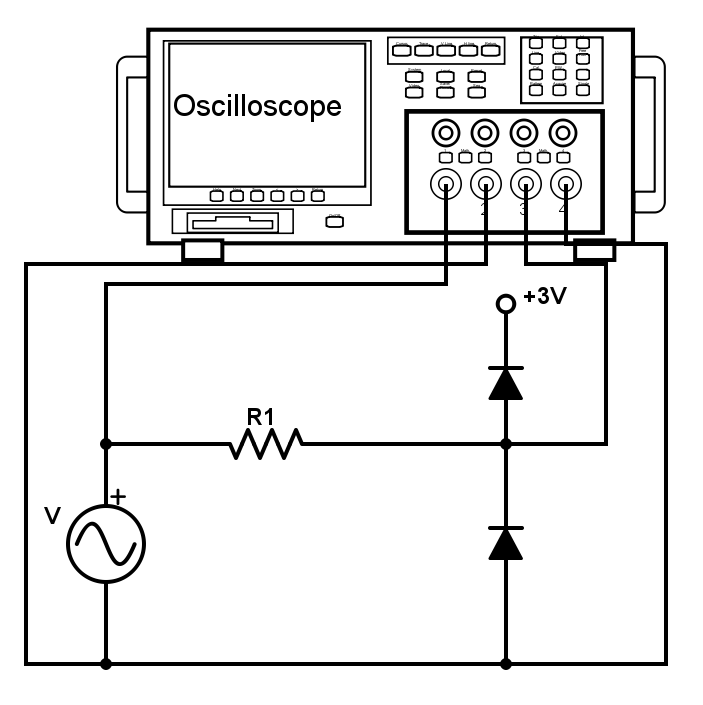
\includegraphics[scale=0.25]{halfwave.png}  
    \caption{This circuit only supplies positive voltage to the oscilloscope.}
\end{figure}

Diodes can also be used to construct a full wave rectifier, shown in figure (2), which allows the positive and negative voltages through while inverting the negative voltage.

\begin{figure}
    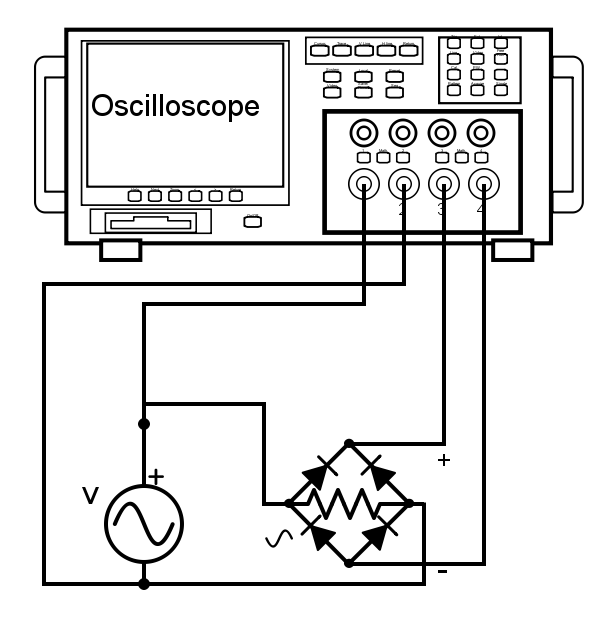
\includegraphics[scale=0.3]{bridge.png}  
    \caption{A full wave rectifier with input and output connected to an oscilloscope}
\end{figure}

The circuit makes all the voltage positive. As positive voltage is supplied, current will pass through the top left diode and not the bottom left because of the orientation of the diode. Current will then flow down through the resistor and not the top right diode. As negative voltage is supplied to the circuit, current will flow from the bottom side of the AC source. As the current flows to the right side of the bridge it will pass through the top right diode and not the bottom right. The current will then flow down through the resistor as it did when a positive voltage was supplied. This combination will cause flow in only one direction through the resistor and the output of the bridge.

Zener diodes are a kind of diode that will allow current to flow in the reverse-bias direction if the voltage is above a certain minimum voltage. This voltage is called the Zener voltage.

\begin{figure}
    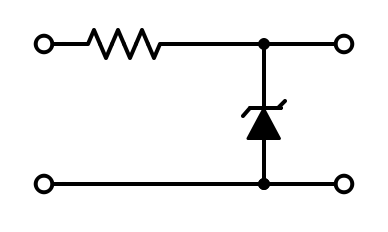
\includegraphics[scale=0.3]{zener.png}  
    \caption{This circuit only supplies positive voltage to the oscilloscope, attached to the right terminals. The power source was connected to the left-side terminals.}
\end{figure}

Zener diodes allow only the Zener voltage to pass 
%One important use of the zener diode was to "clip" the voltage source. This means that the zener diode caps the voltage allowed through... 
%********need to add more when I can see plots******





\section{Methodology}

\begin{enumerate}
    \item Construct RC circuit with oscilloscope as show in figure (1) without the 3V DC source and diode attached.
    \item Take record of the plot from the oscilloscope.
    \item Adjust frequency and amplitude of input source and repeat step 2.
    \item Build diode bridge shown in figure (2).
    \item Connect input source (one that is external from the protoboard) and connect the oscilloscope as shown in figure (2).
    \item Repeat steps 2 and 3 to get data about the bridge.
    \item Construct the circuit shown in figure (3).
    \item Add an adjustable DC input to the left side of the circuit and connect a measurement device to the right side of the circuit.
    \item Make recordings of the output voltages as the input voltage is modified.
    \item Swap the DC input for an AC input and swap the measurement device for one suited for AC voltages (oscilloscope) if necessary.
    \item Take record of the plot shown on the oscilloscope.
    \item Swap the zener diode out for another one and repeat step 11.
    \item Combine the two diodes in series in the same direction and make record of the plot on the oscilloscope.
    \item Combine the two zener diodes in parallel in opposite directions to "clip" both positive and negative voltages from the AC input.
\end{enumerate}


\section{Results and Analysis}

\subsection{Data}
The half wave rectifier was investigated with various input voltages and frequencies. All voltages for $V_{in}$ and $V_{out}$ were maximum voltages.

The input source was initially set to an amplitude of 2.64V and frequency 7.225Hz. The $V_{out}$ measured across the diode was 1.80V.

\begin{figure}[h]
    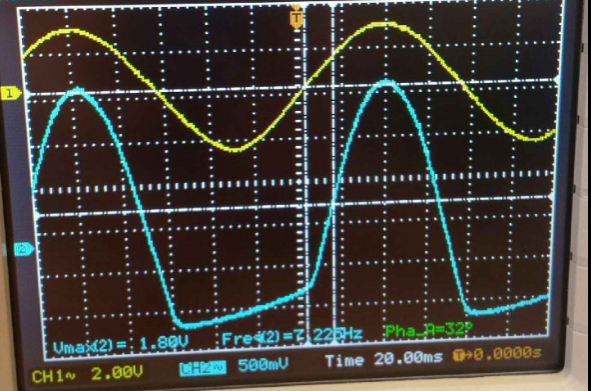
\includegraphics[scale=0.4]{1800mV.png}  
    \caption{$V_{in}= 2.64V$, $f=7.225Hz$, $V_{out} = 1.80V$}
\end{figure}


The group then increased the amplitude of the input voltage to 4.08V. The resulting $V_{out}$ was 2.72V.

\begin{figure}[h]
    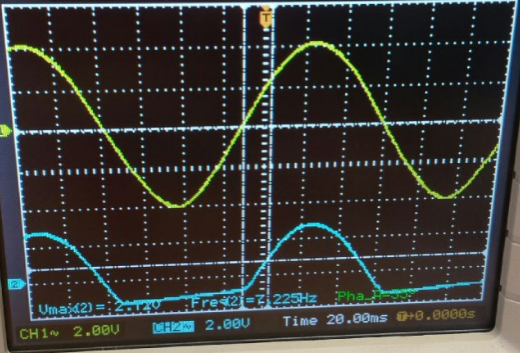
\includegraphics[scale=0.45]{2720mV.png}  
    \caption{$V_{in}= 4.08V$, $f=7.225Hz$, $V_{out}= 2.72V$}
\end{figure}


The group then reset the input voltage to 2.64V and increased the frequency to 75.19Hz. The resulting $V_{out}$ was 1.76V

\begin{figure}[h]
    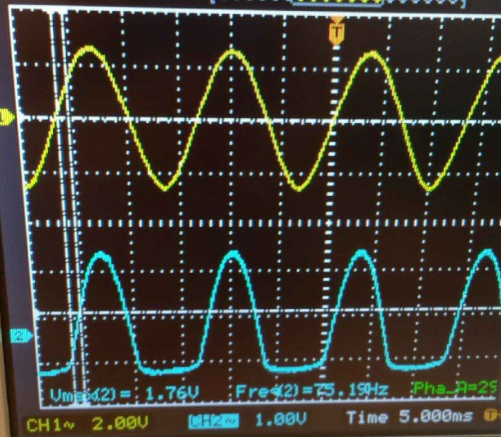
\includegraphics[scale=0.45]{1760mV.png}  
    \caption{$V_{in} = 2.64V$, $f=75.19Hz$, $V_{out}= 1.76V$}
\end{figure}

%fourth frequency: same for higher

The reference voltage added was a 3.065V DC source, constructed in the manner shown in figure (1). 

The input voltage was decreased to 1.48V, and the frequency was set to 7.225Hz. The resulting $V_{out}$ was 460mV.

\begin{figure}[h]
    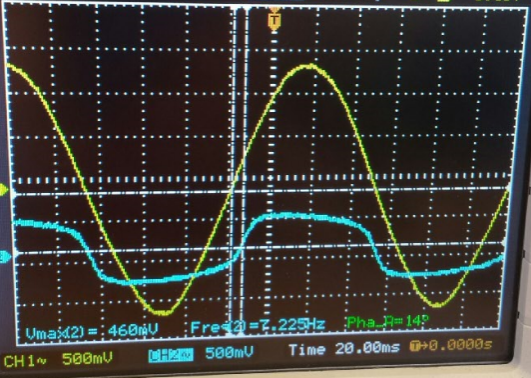
\includegraphics[scale=0.45]{460mV.png}  
    \caption{$V_{in}= 1.48V$, $f=7.225Hz$, $V_{out}= 460mV$}
\end{figure}

%The input voltage and frequency were then set to 2.64V and 731.0mHz respectively. The $V_{out}$ for the diode was 464mV.

%\begin{figure}
%    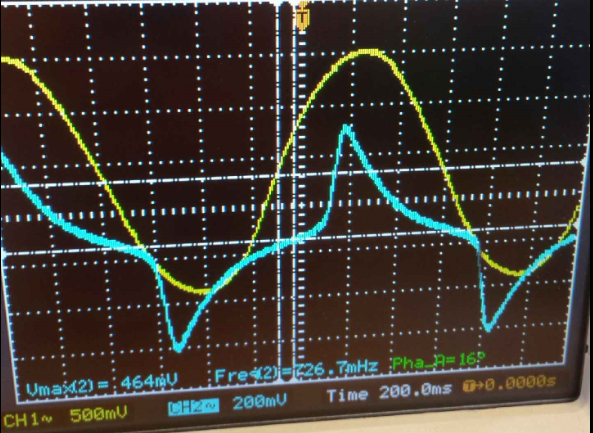
\includegraphics[scale=0.3]{464mV.png}  
%    \caption{$V_{in}$ = 2.64V f=731.0mHz $V_{out}$= 464mV}
%\end{figure}


The group increased the frequency to 74.63Hz and the voltage to 2.64. The resulting $V_{out}$ was 480mV.

\begin{figure}[h]
    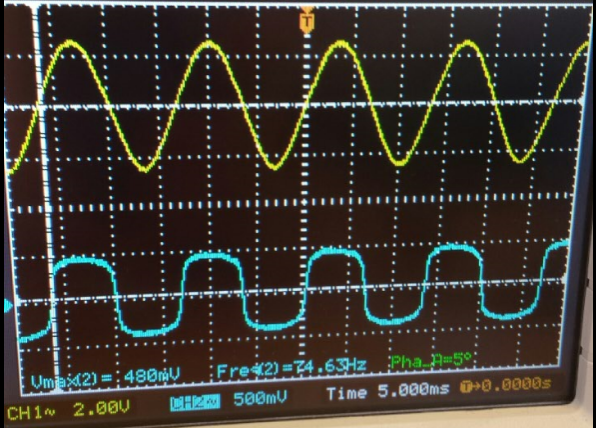
\includegraphics[scale=0.4]{480mV.png}  
    \caption{$V_{in} = 2.64V$, $f=74.63Hz$, $V_{out}= 480mV$}
\end{figure}

The circuit shown in figure (3) was built using a 2.219k$\Omega$ resistor. First, the the Zener diode's behavior was observed as input voltage was varied.
\begin{figure}[h]
    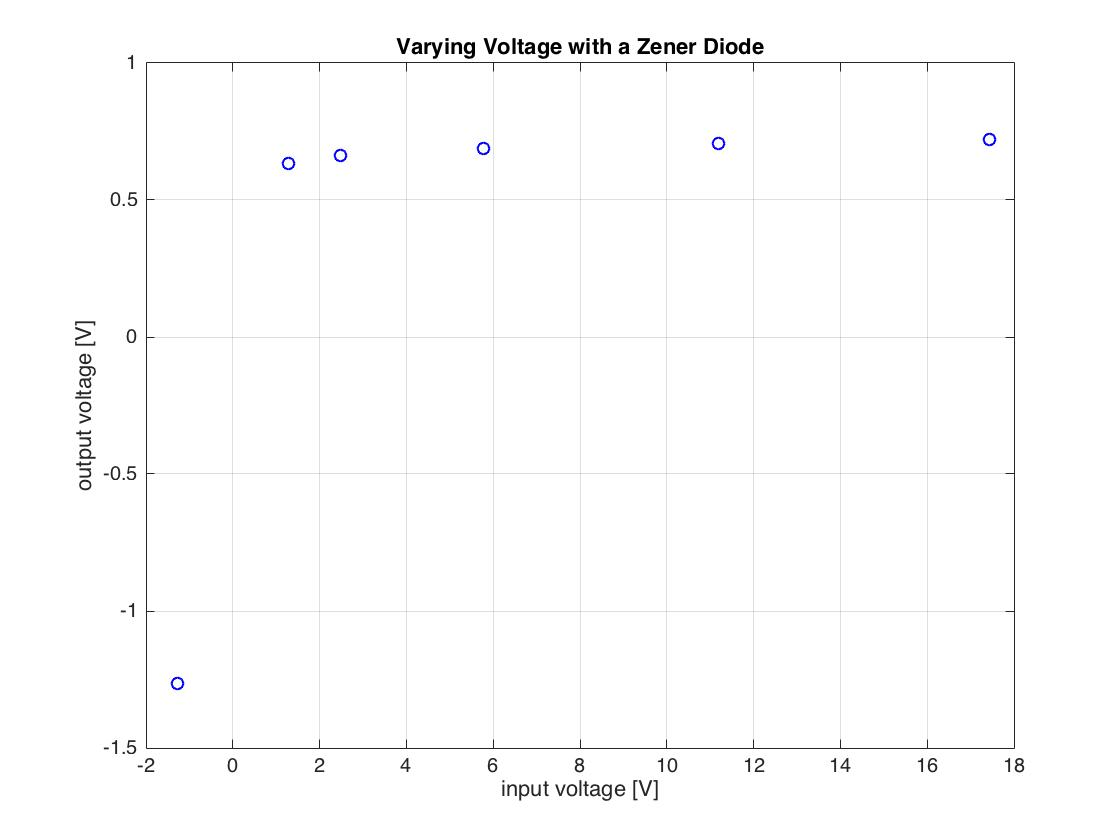
\includegraphics[scale=0.2]{zenerdiode_plot}  
    \caption{Zener diode's response to varying voltage.}
\end{figure}

Two Zener diodes in series in the same direction acted the same as one.

One Zener diode resulted in the clipping of the negative voltage.
\begin{figure}[h]
    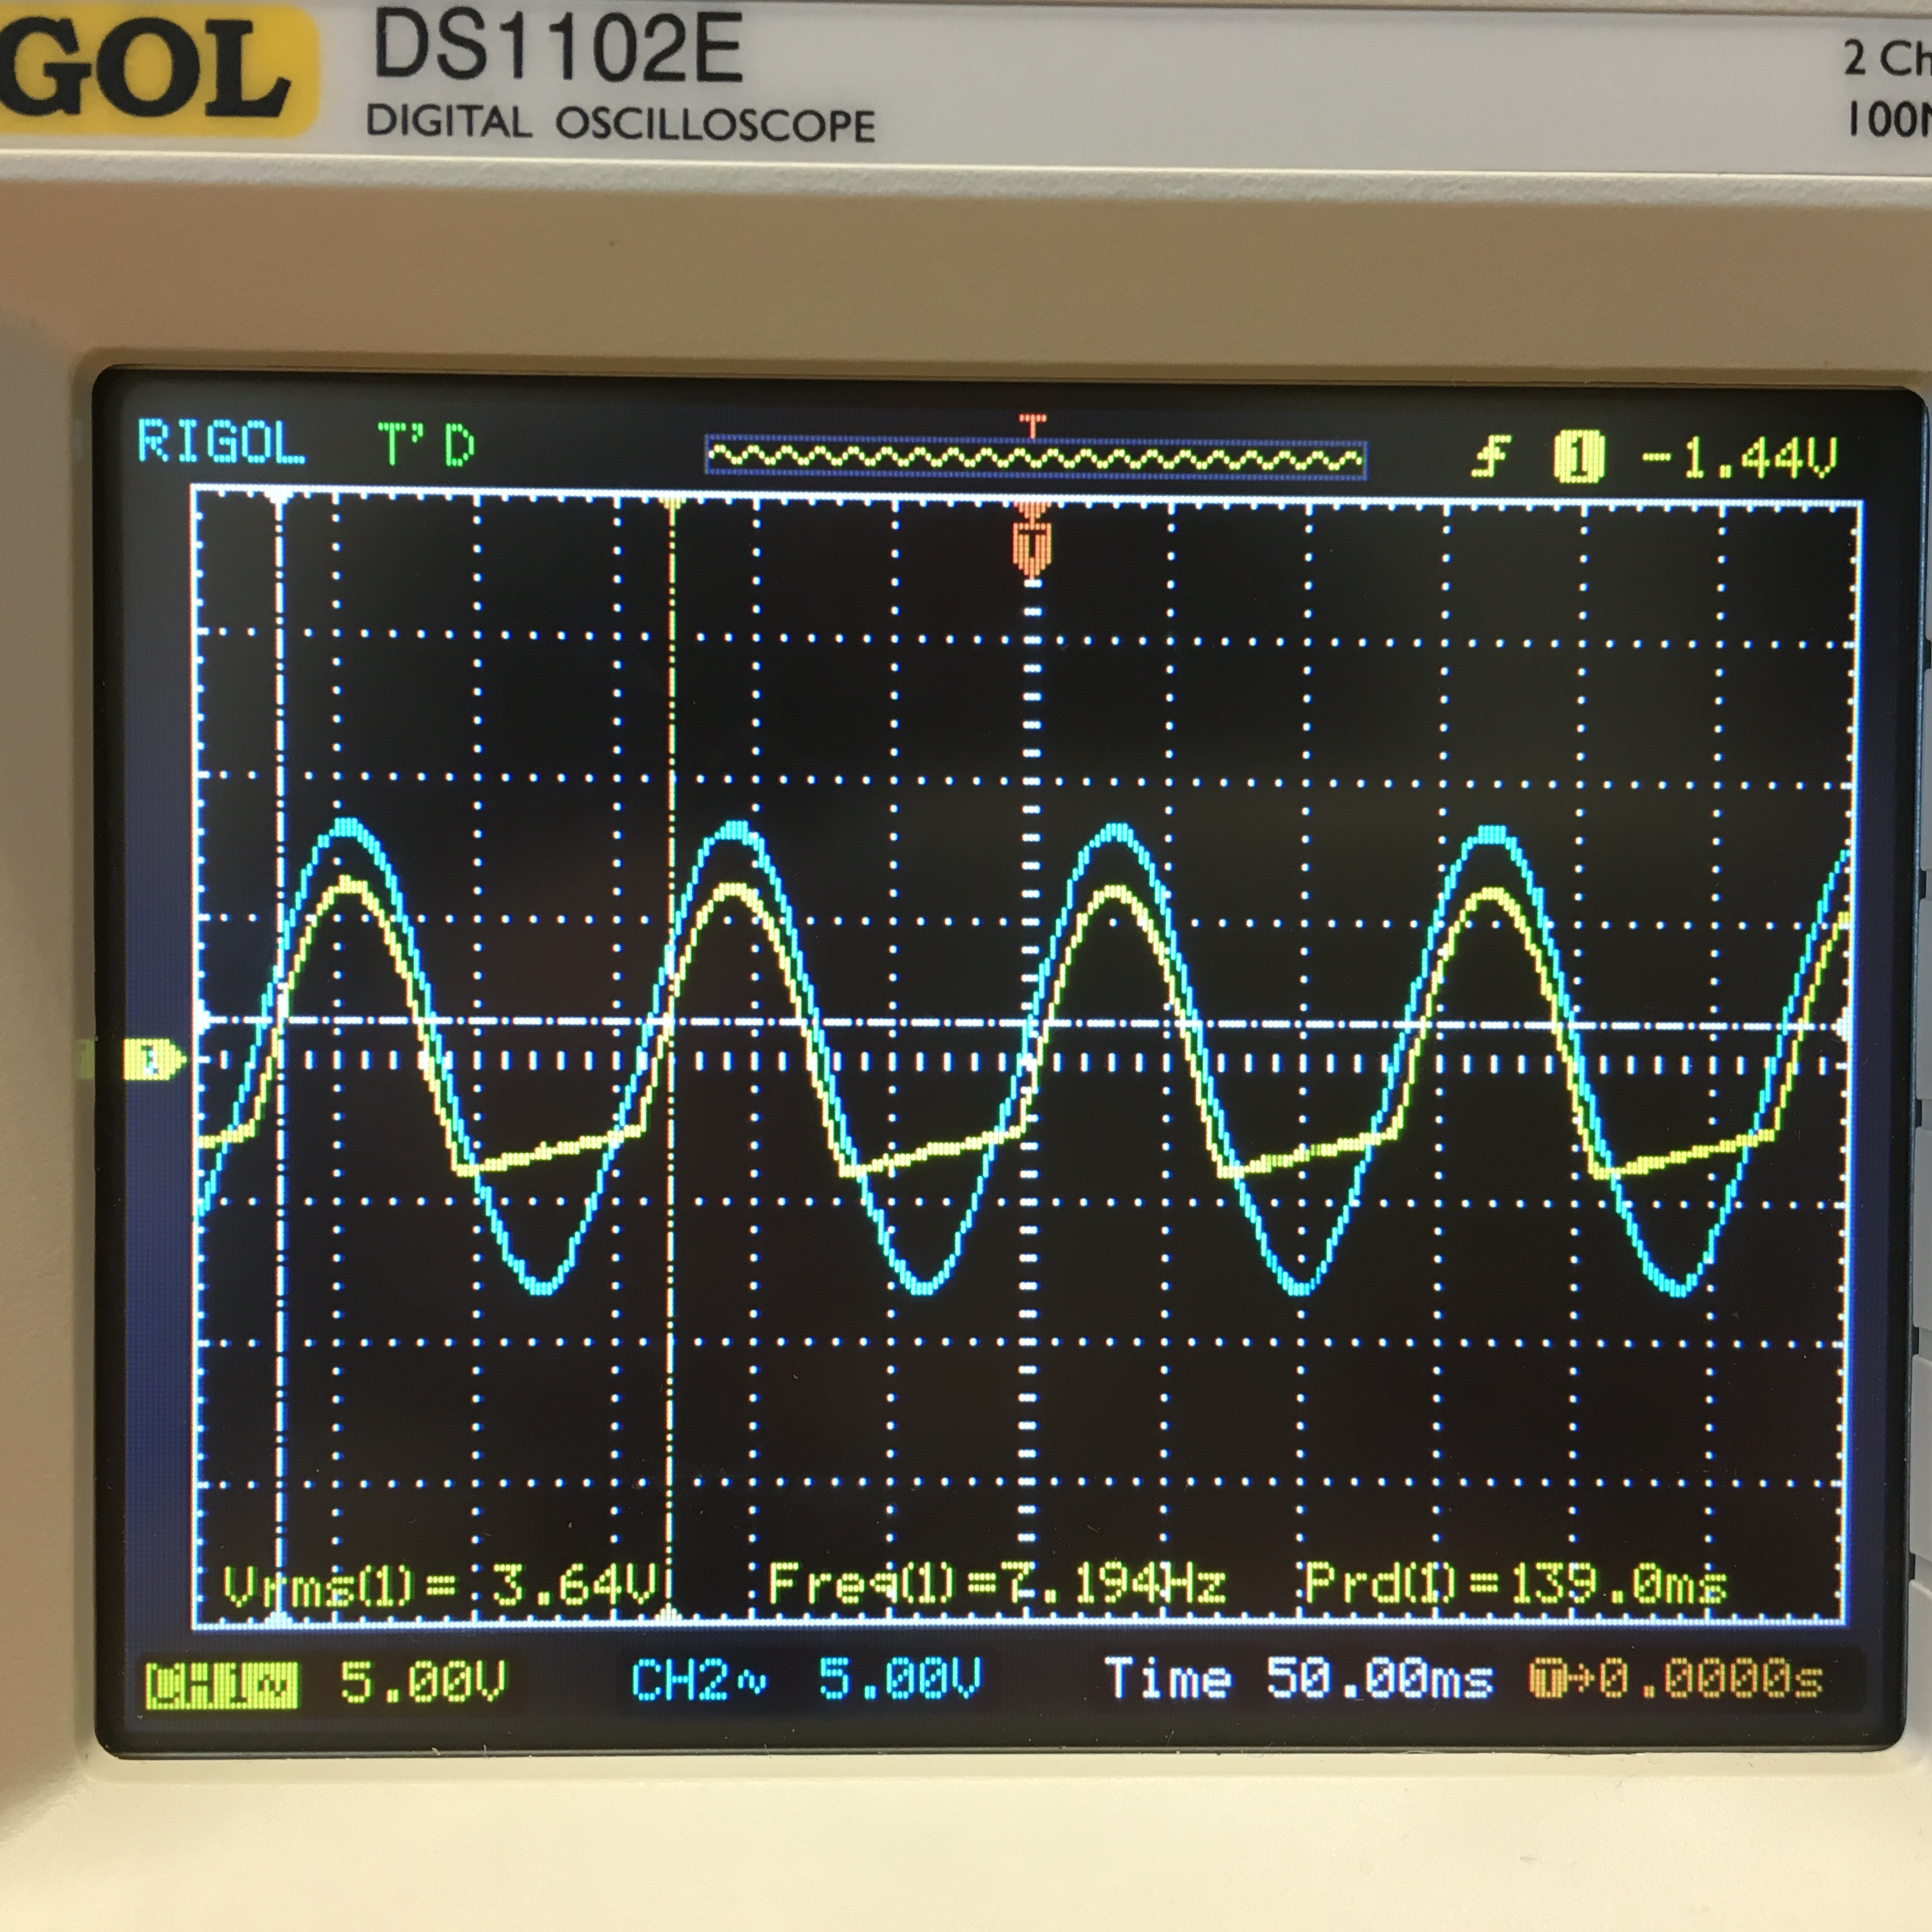
\includegraphics[scale=0.06]{zener2}  
    \caption{Zener diode clipping negative voltage.}
\end{figure}
Two Zener diodes in opposite directions resulted in the clipping of both positive and negative voltages.
\begin{figure}[h]
    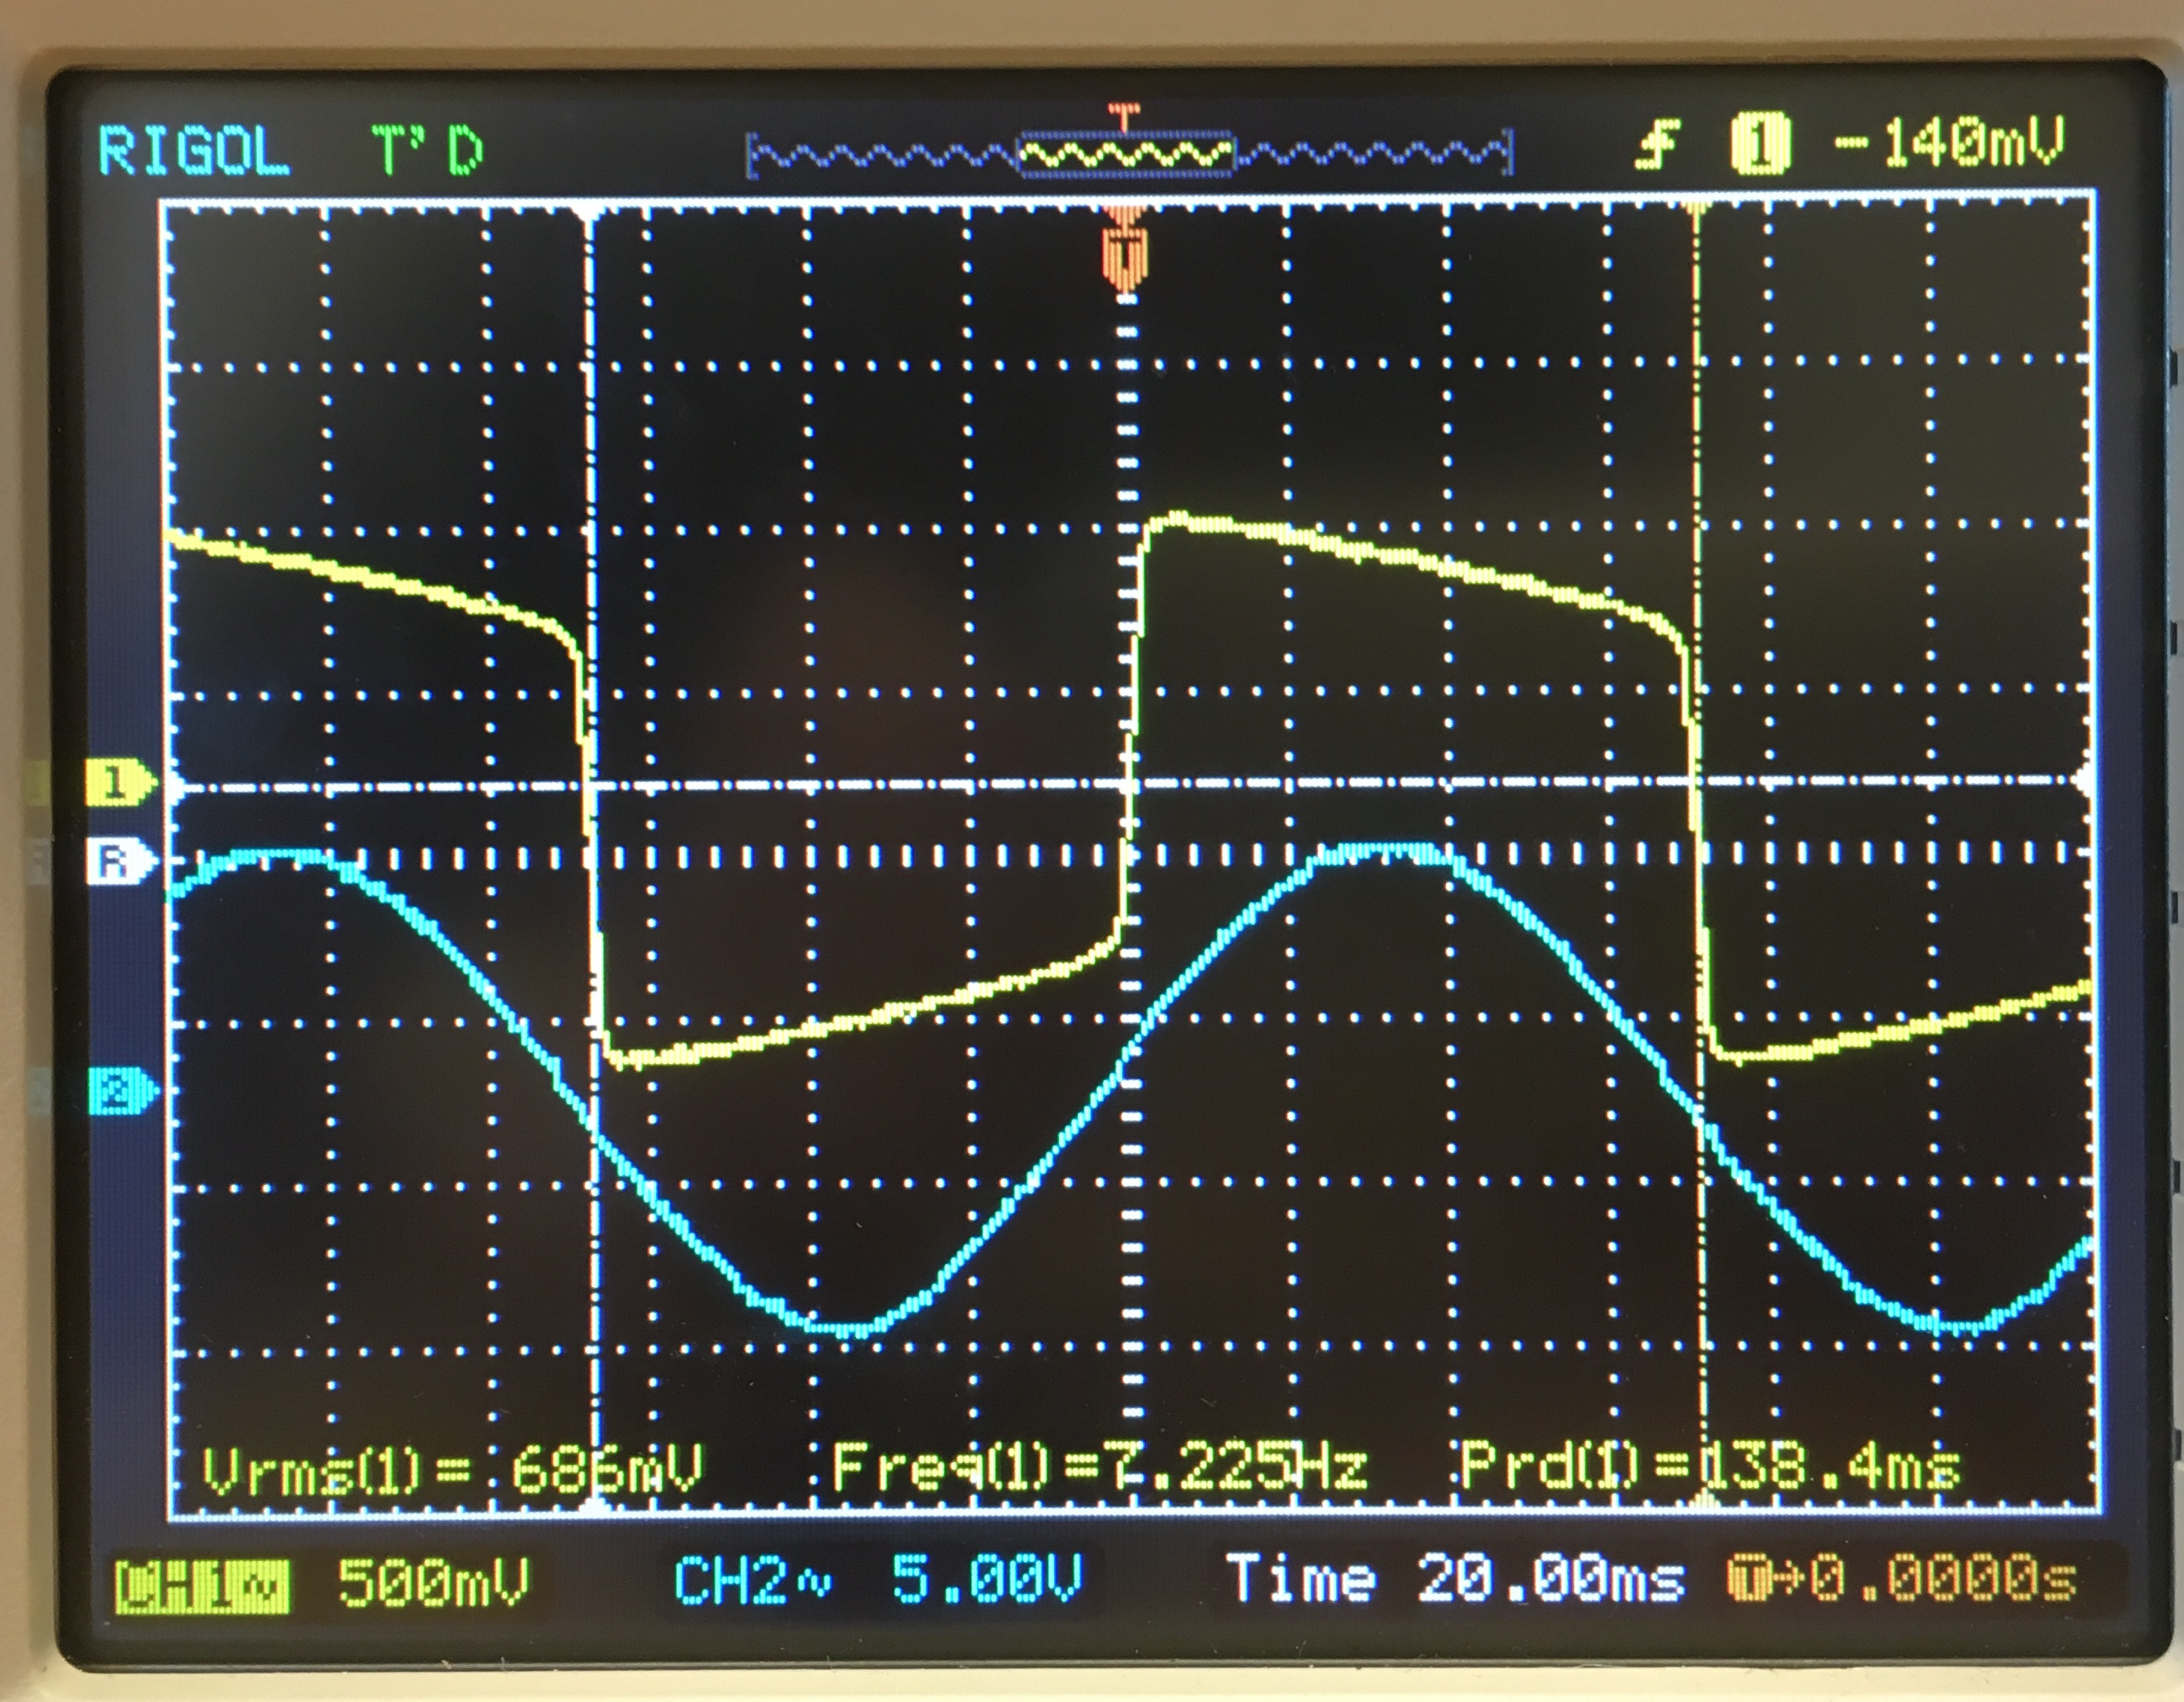
\includegraphics[scale=0.06]{zener1}  
    \caption{Zener diode clipping positive and negative voltage.}
\end{figure}





 
\subsection{Analysis}
When only an AC voltage source was connected to the diode and resistor that were in series, the result was half of a sine wave. This was what was expected because the diode only allows current flow in one direction. The current will flow only in the negative direction which will cause the voltage across the oscilloscope to be equal to the diode voltage. When current cannot flow through the diode almost all of the voltage is across the oscilloscope. This means that when the voltage of the input source is positive the voltage across the oscilloscope is equal to the input voltage. 

When the amplitude of the input source was increased, the slight angle of linear portion of the plots appeared to decrease, as the larger amplitude of the positive curve made the slant relatively smaller.

As the frequency was increased the plot looked almost like a DC source that was turning on and off because the diode voltage was reached faster, reducing the curve on the bottom of the voltage plot.

When the reference voltage was added, the sinusoidal voltage across the diode became flat on top and bottom. When a negative input voltage was supplied, current flowed through the resistor and the voltage across the resistor was equal to the diode voltage. When the voltage of the input source was positive, the 3.065V from the DC source consumed the input voltage. Since the input voltage was never greater than 3V, the output voltage was zero. If the voltage of the input had been greater than 3V, then the voltage across the oscilloscope would have been equal to 3V.

When the frequency was increased, the plot flattened out on top and bottom and looked again like a DC input that was flickering up and down by 480mV. This makes sense as the diode was expected to vary between the diode voltage and zero. When frequency was increased the diode voltage was reached more quickly and therefore makes the plot look flatter.



\section{Conclusion}
The first part of the lab was completed successfully as the group was able to demonstrate that a diode can be used to create close to half of a DC voltage supply. The group discovered that for higher frequency input voltages the plot was more flat on top and bottom. The correct properties of the diode were demonstrated in this part of the lab. When then 3V DC source was added, the results were accurate as the voltage varied between zero and the diode voltage. This is what would have been expected for input voltages below 3V. The mistake of the lab group was not to vary the input voltage much higher to demonstrate that when the voltage supply is greater than 3V, the voltage across the oscilloscope will be capped at 3V. This part of the lab was only partially complete. The results for what was done were as expected. 


\end{document}

